Машинное зрение (Computer Vision, CV) представляет собой область искусственного интеллекта, изучающую методы автоматического анализа изображений и видео с целью извлечения из них семантически значимой информации~\cite{refRakov}. В работе Рублевского~\cite{refRublevsky} машинное зрение выделяется как внешнее кольцо в общей классификации искусственного интеллекта (см. рис.~\ref{fig:classifications_ai}~a).
Машинное зрение включающий задачи обработки документов, выделения структурных областей страницы и распознавания содержащейся на ней информации. Частным направлением компьютерного зрения является анализ изображений документов (Document Image Analysis или Document Understanding)(см.~рис.~\ref{fig:classifications_ai}~b), в рамках которого решаются задачи сегментации страницы, распознавания текста, таблиц, графики и иных содержательных элементов~\cite{refLayoutParser,refLayoutLM}.

Одной из наиболее известных задач данного направления является OCR (optical character recognition, оптическое распознавание символов), ориентированная на извлечение текстовой информации из изображений документов~\cite{refSmith}. Однако, как было сказано, в химической литературе значимая часть информации представлена не только текстом, но и графическими структурами, поэтому наряду с OCR требуется использовать специализированные методы OCSR (optical chemical structure recognition, оптическое распознавание химической структур)~\cite{refWikiOCSR}, предназначенные для восстановления химических структур по их изображению. С методологической точки зрения OCSR не сводится к обычному OCR, поскольку предполагает восстановление молекулярного графа, а не только линейной последовательности символов. Таким образом, OCR и OCSR целесообразно рассматривать как родственные, но не вложенные подзадачи анализа изображений химических документов (см.~рис.~\ref{fig:classifications_ai}~b).


\begin{figure*}[hbtp]
	\centering
	\begin{tabular}{cc}
		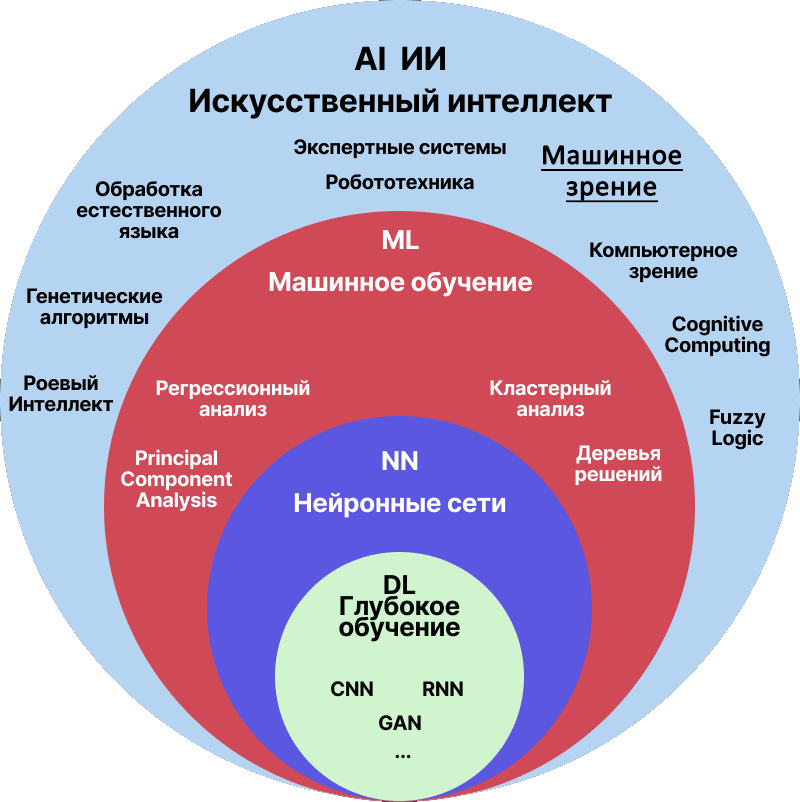
\includegraphics[width=0.45\linewidth]{img/classifications_ai.png} &
		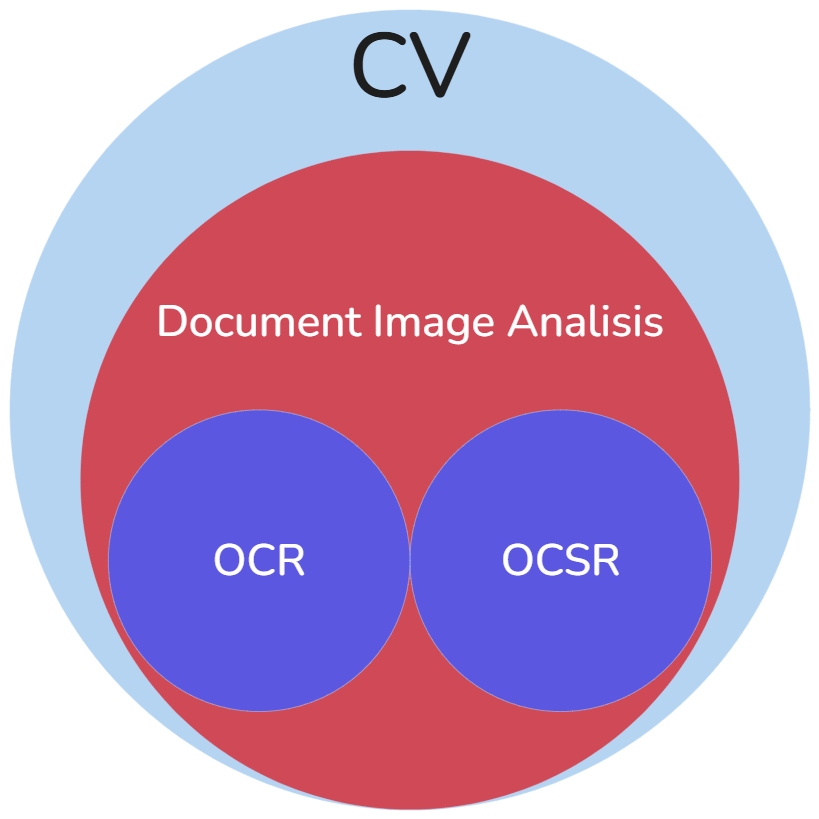
\includegraphics[width=0.45\linewidth]{img/classifications_cv.png} \\
		a$)$ & b$)$
	\end{tabular}
	\bicaption
	{
		а) Классификация искусственного интеллекта;
		b) Классификация компьютерного зрения.
	}
	{
		a) Classification of artificial intelligence;
		b) Classification of computer vision.
	}
	\label{fig:classifications_ai}
\end{figure*}